\section{Taust}
Masinõppemeetodite tulemuslikkuse mõõtmiseks kasutatakse mitmeid teoreetilisi kvaliteedimõõtusid.
Kvaliteedimõõdud on defineeritud läbi nende ooteväärtuste. Praktikas hinnatakse kvaliteedimõõtusid ligikaudselt, arvutades keskmisi väärtusi üle valimi.

\subsection{Lõplikud ja lõpmatud andmekogumid}
Statistilises uuringus nimetatakse uuringu all olevat objekti üldkogumiks ehk populatsiooniks.
Populatsioon koosneb andmepunktidest. Andmepunktide kogus on määratletud populatsiooni korral tavaliselt lõplik. Kõikse uuringu korral mõõdetakse kõiki populatsiooni andmepunkte. Kõikne uuring on sageli ülemäära kulukas. Lihtsam on mõõta juhuslikku osahulka populatsiooni andmepunktidest. Mõõdetavate andmepunktide hulka nimetatakse valimiks. Valimi põhjal tehakse järeldusi kogu populatsiooni kohta. Tehtud järeldused võivad valimi juhuslikkuse tõttu sisaldada vigu, kuid sellised vead on tõenäosuslikult hinnatavad \cite{rakendusstatisika-algkursus}.

Vahel pole populatsioon uuringu tegemise hetkel üheselt fikseeritud või lõplik, nagu näiteks kõik järgmise 24 tunni jooksul kiirabisse pöörduvad inimesed või kõigi Canon 70D fotokaameratega tehtud pildid. Sellisel juhul määrab tulemuse andmeid genereeriv füüsiline protsess ning seda mudeldatakse tihti juhusliku jaotusega. Formaalselt on juhuslik jaotus andmete allikas, millest saab võtta kuitahes palju sõltumatuid andmepunkte. Antud töös vaatame protsesse, millel on lõplik arv väljundväärtusi, see tähendab jaotus on diskreetne. Sel juhul fikseerib jaotus iga konkreetse andmepunkti jaoks selle esinemistõenäosuse, millest võib mõelda kui andmepunkti oodatavat sagedusest valimis, millesse on võetud piisavalt palju andmepunkte jaotusest. 

Lõpliku valimi korral saab mingi uuritava omaduse $A$ esinemise tõenäosust defineerida kui suhet omaduse esinemise arvu valimis $n_A$ ning valimi suuruse $n$ vahel
\begin{equation*}
    \prob{A}=\frac{n_A}{n} \enspace.
\end{equation*}
Juhuslikust valimist juhusliku andmepunkti võtmiselt tähendab see tõenäosust, et andmepunkt on omadusega $A$.

Juhuslikku valimit saab moodustada võttes populatsioonist andmepunkte üksteisest sõltumatult ja juhuslikult. Võib juhtuda, et samad populatsiooni andmepunktid sattuvad valimisse mitmekordselt. Saadud valimi puhul eeldatakse, et kõik selle andmepunktid on sama jaotusega. Tegelikkuses ei pruugi sõltumatuse ja sama jaotuse eeldus olla täidetud. Näiteks Canon 70D fotokaameraga tehtud pildiseeria piltide jaotused on üksteisega korreleeritud, kuna  ühest sündmusest tehakse tavaliselt mitu pilti. See-eest üksikute piltide jaotuste puhul võib sageli sõltumatust eeldada. Valimikeskmine on valimi kõikide andmepunktide väärtuste aritmeetiline keskmine
\begin{equation}
    \label{eq:valimikeskmine}
    \bar{x}=\frac{1}{n}\cdot\sum_{i = 1}^{n}x_i \enspace.
\end{equation}
Juhul kui $x_i$ on indikaator valimi $i$-nda andepunkti mingi omaduse kohta, läheneb valimikeskmine $\bar{x}$ tõenäosusele, et juhuslikul objektil on see omadus.

Valimidispersioon on kõigi andmepunktide hälvete ruutude aritmeetiline keskmine
\begin{equation}
    \label{eq:nihkega valimidispersioon}
    s^2=\frac{1}{n}\cdot\sum_{i=1}^{n}(x_i-\bar{x})^2 \enspace.
\end{equation}
Dispersioon näitab andmete hajuvust. Valimidispersiooni kaudu saab leida hinnangu valimikeskmise dispersioonile $\frac{s^2}{n}$, millest ruutjuurt nimetatakse standardveaks \cite{rakendusstatisika-algkursus}. Standardviga näitab valimikeskmise $\bar{x}$ fluktuatsiooni tema oodatud väärtusest, ehk mitut tüvenumbrit hinnangust võib usaldada.

Olgu olemas juhuslik protsess, mis genereerib populatsiooni andmepunkte. Protsessi genereeritud andmepunktid on üksteisest sõltumatud ja sama jaotusega. Jaotuse abil defineeritud potentsiaalselt lõpmatu andmestiku uurimiseks saab defineerida valimiüleste valemite \eqref{eq:valimikeskmine} ja \eqref{eq:nihkega valimidispersioon} analoogid, milleks need lõpmata suure valimi korral koonduvad.

Valimikeskmise analoog keskväärtus iseloomustab jaotuse väärtuste paiknevust, mõnikord nimetatakse keskväärtust ka matemaatiliseks ootuseks \cite{tõenäosusteooria-algkursus}. Diskreetse juhusliku suuruse $X$ keskväärtus on defineeritud summana
\begin{equation}
    \label{eq:keskväärtus}
    \mean{X}=\sum_{i}x_i p_i \enspace,
\end{equation}
kus $x_i$ on suuruse üks võimalik väärtus ning $p_i$ tõenäosus, et $X$ selle väärtuse võtab. Pideva juhusliku suuruse $X$, mille tihedusfunktsioon on $f_X(x)$, keskväärtus leitav määratud integraalina
\begin{equation*}
    \mean{X}=\int_{-\infty}^{\infty}x\cdot f_X(x)\,dx \enspace,
\end{equation*}
mitmemõõtmelise juhusliku suuruse korral on selle keskväärtus leitav analoogiliselt mitmemõõtmelise integraaliga.

Valimidispersiooni analoog dispersioon on juhusliku suuruse hälve ruudu keskväärtus
\begin{equation}
    \label{eq:dispersioon}
    \variance{X}=\mean{(X-\mean{X})^2}=\mean{X^2}-\mean{X}^2 \enspace.
\end{equation}
Ruutjuurt dispersioonist nimetatakse standardhälbeks. Lõpliku populatsiooni korral avalduvad jaotuseülesed valemid \eqref{eq:keskväärtus} ja \eqref{eq:dispersioon} neile vastavate valimiüleste valemitena \eqref{eq:valimikeskmine} ja \eqref{eq:nihkega valimidispersioon}. Jaotuseülesed valemeid on vaja, et uurida juhuslikkust sisaldavate suuruste oodatud käitumist.

\subsection{Veahinnangud}
\label{section:veahinnangud}
Numbriliselt ülesannete lahendamisel võib täpse lahendi leidmine olla aeganõudev ja kulukas.
Ülesande ligikaudne lahendamine võib osutuda otstarbekamaks, näiteks populatsiooni keskväärtuse leidmise asemel leida valimikeskmine. Antud näite korral on valimikeskmine ligikaudne hinnang keskväärtusele. Ligikaudsete väärtuste headust on võimlaik mõõta kasutades veahinnanguid. Veahinnangud kirjeldavad mingi täpse arvu ja selle lähendi erinevust. Vastuse lähendamisel praktilises olukorras ei pruugi olla täpset lahendust teada. Seega sobivad veahinnangud lähendamismeetodite teoreetiliseks hindamiseks.

Olgu $a$ ligikaudne väärtus arvust $a_0$. Ligikaudse arvu $a$ absoluutseks veaks nimetatakse arvu
\begin{equation*}
    \Delta a=a-a_0 \enspace.
\end{equation*}
Absoluutse vea õigesti mõistmiseks tuleb arvestada lähendatava arvu skaalaga. Arvude puhul, mis ulatuvad mitmetesse tuhandetesse, tähendab absoluutne viga $0{,}5$ väga täpset lähendit. Nulli ja ühe vaheliste arvude puhul mitte. Seevastu saab kasutusele võtta hinnangu, mis arvestab skaalaga. Ligikaudse arvu $a$ relatiivseks ehk suhteliseks veaks nimetatakse suurust
\begin{equation*}
    \delta a=\frac{\Delta a}{a_0}=\frac{a-a_0}{a_0}=\frac{a}{a_0}-1 \enspace.
\end{equation*}
Mõnikord esitatakse relatiivne viga protsentides.

Ligikaudsete väärtuste puhul on eesmärgiks nende veahinnangute absoluutväärtuselt minimeerimine. Alati ei pruugi see olla võimalik, tuleb leppida mingi veaga. Lisaks võib raske olla täielikult veenduda, et leitud lähendi viga on väiksem kui maksimaalne lubatud viga. See-eest võib võimalik olla uurida kui suure tõenäosusega on saavutatud viga, mis on väiksem lubatud maksimaalsest veast
\begin{equation*}
    \prob{\mid a - a_0 \mid < \varepsilon} = 1 - \alpha \enspace,
\end{equation*}
kus $\varepsilon$ on absoluutse vea absoluutväärtuse ülemine piir, suurust $\alpha$ nimetatakse olulisusnivooks ning vahet $1-\alpha$ usaldusnivooks või kindluseks. Tihti valitakse $\alpha$ väärtuseks $0{,}05$, mõnikord ka $0{,}01$ või isegi $0{,}32$.

Kui juhuslik suurus on vaadeldav paljude sõltumatute juhuslike suuruste summana on alust arvata, et summa on ligikaudu normaaljaotusega \cite{tõenäosusteooria-algkursus}. Seega kui ligikaudsed väärtused sisaldavad paljude sõltumatute juhuslike veakomponentide summat võib ka veahinnangute puhul eeldada, et need on normaaljaotusega.

Juhuslik suurus $X$ on normaaljaotusega kui tema tihedusfunktsioon on
\begin{equation*}
    f_X(x)=\frac{1}{\sqrt{2\pi}\sigma}\cdot\exp{\left(-\frac{(x-\mu)^2}{2\sigma^2}\right)} \enspace,
\end{equation*}
kus jaotuse parameetrid $\mu$ ja $\sigma$ on vastavalt $X$ keskväärtus ja standardhälve. Seda fakti tähistatakse lühidalt $X\sim\mathcal{N}(\mu,\sigma)$. Normaaljaotuse tihedus on sümmeetriline keskväärtuse $\mu$ ümber. Veahinnangute puhul on nende oodatud väärtus null, siis sümmeetrilisuse tõttu on negatiivsed ja positiivsed vead sama tõenäolised. Oluline omadus normaaljaotuse puhul on see, kui suure tõenäosuse katavad standardhälbe täisarvkordsed vahemikud keskväärtuse ümbruses. Vahemik $\mu\pm\sigma$ katab tõenäosuse $68\%$, $\mu\pm2\sigma$ tõenäosuse $95\%$ ning $\mu\pm3\sigma$ tõenäosuse $99\%$.

\subsubsection{Summa ja vahe relatiivse vea omadus}
Vahel võib uuritav suurus olla arvutatav mitme ligikaudse suuruse kaudu. Ligikaudsete suurustega tehtud arvutused annavad ligikaudseid tulemusi. Seega tasub tulemuse täpsuse hindamiseks uurida kuidas viga arvutustel edasi kandub. Sealjuures tehakse tihti lihtsustav eeldus, et lähendid on normaaljaotusega.

Olgu $x$ ja $y$ ligikaudsed väärtused arvudest $x_0$ ja $y_0$ absoluutsete vigadega vastavalt $\varepsilon_x$ ning $\varepsilon_y$:
\begin{align*}
    x&=x_0+\varepsilon_x ,\qquad \varepsilon_x\sim\mathcal{N}(0, \sigma_x) \enspace,\\
    y&=y_0+\varepsilon_y ,\qquad \varepsilon_y\sim\mathcal{N}(0, \sigma_y) \enspace,
\end{align*}
kus vead $\varepsilon_x$ ja $\varepsilon_y$ on sõltumatud. Ligikaudsete väärtuste $x$ ja $y$ summa relatiivne viga avaldub kujul
\begin{equation*}
    \delta_{+}=\frac{(x+y)-(x_0+y_0)}{x_0+y_0}=\frac{x_0+\varepsilon_x+y_0+\varepsilon_y-x_0-y_0}{x_0+y_0}=\frac{\varepsilon_x+\varepsilon_y}{x_0+y_0} \enspace.
\end{equation*}
Kuna $\varepsilon_x$ ja $\varepsilon_y$ keskväärtused on nullid on ka summa relatiivse vea $\delta_{+}$ keskväärtus null. Vigade sõltumatuse tõttu on korrutise $\varepsilon_x\cdot\varepsilon_y$ keskväärtus samuti null. Seega on summa relatiivse vea hajuvus leitav kui selle ruudu keskväärtus
\begin{align*}
    \variance{\delta_{+}}&=\mean{\delta_{+}^2}=\mean{\frac{\varepsilon_x^2+2\varepsilon_x\varepsilon_y+\varepsilon_y^2}{(x_0+y_0)^2}} 
    &=\mean{\frac{\varepsilon_x^2+\varepsilon_y^2}{(x_0+y_0)^2}}=\frac{\variance{\varepsilon_x}+\variance{\varepsilon_y}}{(x_0+y_0)^2} \enspace.
\end{align*}

Ligikaudsete arvude $x$ ja $y$ vahe relatiivne viga avaldub sarnaselt summale
\begin{align*}
    \delta_{-}&=\frac{\varepsilon_x-\varepsilon_y}{x_0-y_0} \enspace.
\end{align*}
Vahe relatiivse vea dispersioon on kujult samuti sarnane summale, kuid juhul kui täpsed väärtused on lähedased on selle hajuvus väga suur
\begin{align*}
    \variance{\delta_{-}}&=\frac{\variance{\varepsilon_x}+\variance{\varepsilon_y}}{(x_0-y_0)^2} \enspace.
\end{align*}

\begin{figure}[H]
    \begin{center}
        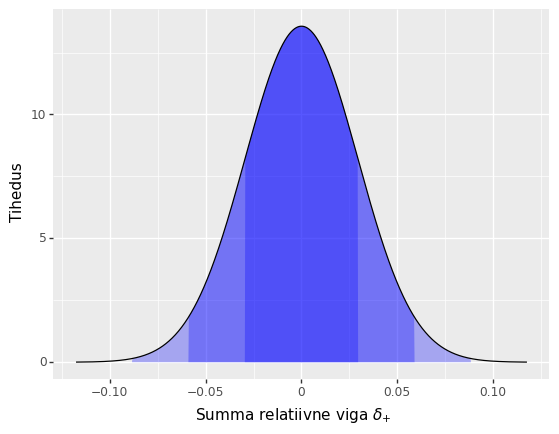
\includegraphics[width=0.8\textwidth]{summa_relatiivne_viga_tihedus.png}
    \end{center}
    \caption{Summa relatiivse vea tihedus juhul $x\sim\mathcal{N}(0{,}8; 0{,}04)$, $y\sim\mathcal{N}(0{,}9; 0{,}03)$.}
    \label{fig:summa relatiivne viga tihedus}
\end{figure}

Kuna veakomponentide $\varepsilon_x$ ja $\varepsilon_y$ puhul on eeldatud normaaljaotust, on võimalik normaaljaotuse omadusi kasutades arvutada, mis tõenäosusega viga $\delta_{+}$ või $\delta_{-}$ mingisse vahemikku jääb.
Näiteks täpsete väärtuste $x_0=0{,}8$, $y_0=0{,}9$ ning absoluutsete vigage $\varepsilon_x\sim\mathcal{N}(0; 0{,}04)$, $\varepsilon_y\sim\mathcal{N}(0; 0{,}03)$ korral jääb $x+y$ relatiivne viga tõenäosusega ligikaudu $68\%$ vahemikku $\pm0{,}029$.
Joonisel \ref{fig:summa relatiivne viga tihedus} on kujutatud antud näite korral summa $x+y$ relatiivse vea tihedus. Heledusega esiletõstetud alad märgivad standardhälbe täisarvkordseid vahemikke keskväärtuse ümber.

\subsubsection{Korrutise relatiivse vea omadus}
Mõnikord võib lähendatav suurus olla leitav ligikaudsete arvude korrutisena. Näiteks riskülikukujulise põranda pindala leidmiseks peab korrutama põranda laiuse ja pikkuse, mis mõõtemääramatuse või vigase mõõteriista tõttu ei pruugi olla täpsed.

Olgu $x$ ja $y$ ligikaudsed väärtused arvudest $x_0$ ja $y_0$ absoluutsete vigadega vastavalt $\varepsilon_x$ ning $\varepsilon_y$:
\begin{align*}
    x&=x_0+\varepsilon_x ,\qquad \varepsilon_x\sim\mathcal{N}(0, \sigma_x) \enspace,\\
    y&=y_0+\varepsilon_y ,\qquad \varepsilon_y\sim\mathcal{N}(0, \sigma_y) \enspace,
\end{align*}
kus vead $\varepsilon_x$ ja $\varepsilon_y$ on sõltumatud. Suuruste $x$ ja $y$ korrutise relatiivne viga avaldub kujul
\begin{align*}
    \delta&=\frac{x\cdot y-x_0\cdot y_0}{x_0\cdot y_0}=\frac{(x_0+\varepsilon_x)\cdot(y_0+\varepsilon_y)-x_0\cdot y_0}{x_0\cdot y_0} \\
    &=\frac{x_0\cdot\varepsilon_y+y_0\cdot\varepsilon_x+\varepsilon_x\cdot\varepsilon_y}{x_0\cdot y_0}=\frac{\varepsilon_y}{y_0}+\frac{\varepsilon_x}{x_0}+\frac{\varepsilon_x}{x_0}\cdot\frac{\varepsilon_y}{y_0} \enspace.
\end{align*}
Vigade $\varepsilon_x$ ja $\varepsilon_y$ sõltumatuse tõttu on $\delta$ keskväärtus null. Arvestades eelnevat saab tuletada korrutise relatiivse vea dispersiooni
\begin{align*}
    \variance{\delta}&=\mean{\delta^2}-\mean{\delta}^2=\mean{\delta^2}-0 \\
    &=\mean{\left(\frac{\varepsilon_y}{y_0}\right)^2 + \left(\frac{\varepsilon_x}{x_0}\right)^2 + \left(\frac{\varepsilon_x}{x_0}\cdot\frac{\varepsilon_y}{y_0}\right)^2 + 2\cdot\frac{\varepsilon_x\cdot\varepsilon_y}{x_0\cdot y_0} + 2\cdot\frac{\varepsilon_x^2\cdot\varepsilon_y}{x_0^2\cdot y_0} + 2\cdot\frac{\varepsilon_x\cdot\varepsilon_y^2}{x_0\cdot y_0^2}} \\
    &=\mean{\left(\frac{\varepsilon_y}{y_0}\right)^2+\left(\frac{\varepsilon_x}{x_0}\right)^2+\left(\frac{\varepsilon_x}{x_0}\cdot\frac{\varepsilon_y}{y_0}\right)^2} \\
    &=\variance{\frac{\varepsilon_y}{y_0}}+\variance{\frac{\varepsilon_x}{x_0}} +\variance{\frac{\varepsilon_y}{y_0}}\cdot\variance{\frac{\varepsilon_x}{x_0}} \enspace.
\end{align*}
Kui $x$ ja $y$ relatiivsete vigade dispersioonid on väikesed on nende korrutis veelgi väiksem. Sellisel juhul saab $\delta$ dispersiooni hinnata küllaltki täpselt jättes korrutise arvutusest välja
\begin{equation}
    \label{eq:korrutise relatiivne viga dispersioon ligikaudne}
    \variance{\delta}\approx\variance{\frac{\varepsilon_y}{y_0}}+\variance{\frac{\varepsilon_x}{x_0}} \enspace.
\end{equation}

\begin{figure}[H]
    \begin{center}
        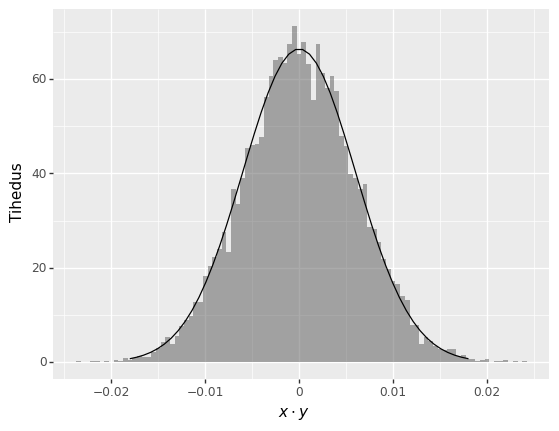
\includegraphics[width=0.8\textwidth]{joonised/korrutis_relatiivne_viga.png}
    \end{center}
    \caption{Korrutise $x\cdot y$ relatiivse vea simuleeritud tihedus histogrammina ja teoreetiline lähendus normaaöjaotsega juhul $x\sim\mathcal{N}(0{,}8; 0{,}004)$, $y\sim\mathcal{N}(0{,}9; 0{,}003)$.}
    \label{fig:korrutis relatiivne viga tihedus}
\end{figure}

Joonisel \ref{fig:korrutis relatiivne viga tihedus} on histogrammina esitatud simuleeritud korrutise $x\cdot y$ relatiivne viga kümnetuhande juhusliku $x$ ja $y$ väärtuse puhul, kus $x\sim\mathcal{N}(0{,}8; 0{,}004)$, $y\sim\mathcal{N}(0{,}9; 0{,}003)$. Tumeda joonega on näidatud korrutise relatiivse vea lähendus normaaljaotusega tulemuse \eqref{eq:korrutise relatiivne viga dispersioon ligikaudne} põhjal.

\subsubsection{Jagatise relatiivse vea omadus}
Osutub, et jagatise puhul on vea edasikandumine natukene keerulisem. Mõningatel eeldustel on leitav piisavalt täpne hinnang jagatise relatiivse vea kohta.

Olgu $x$ ja $y$ ligikaudsed väärtused arvudest $x_0$ ja $y_0$ absoluutsete vigadega vastavalt $\varepsilon_x$ ning $\varepsilon_y$:
\begin{align*}
    x&=x_0+\varepsilon_x ,\qquad \varepsilon_x\sim\mathcal{N}(0, \sigma_x) \enspace,\\
    y&=y_0+\varepsilon_y ,\qquad \varepsilon_y\sim\mathcal{N}(0, \sigma_y) \enspace,
\end{align*}
kus vead $\varepsilon_x$ ja $\varepsilon_y$ on sõltumatud. Suuruste $x$ ja $y$ jagatise relatiivne viga avaldub kujul
\begin{equation*}
    \delta=\biggl(\frac{x}{y}-\frac{x_0}{y_0}\biggr):\frac{x_0}{y_0}=\frac{x\cdot y_0}{y\cdot x_0}-1=\frac{y_0}{x_0}\cdot\frac{x_0+\varepsilon_x}{y_0+\varepsilon_y}-1 \enspace.
\end{equation*}
Jagatise relatiivse vea dispersiooni leidmist saab taandada korrutise relatiivse vea dispersioonile, sest $x/y=x\cdot y^{-1}$. Seega on vaja hinnata $y$ pöördväärtuse relatiivse vea disperisooni
\begin{equation}
    \label{eq:1/y relatiivne viga dispersioon}
    \variance{\left(\frac{1}{y}-\frac{1}{y_0}\right):\frac{1}{y_0}}=\variance{\frac{y_0}{y}}=y_0^2\cdot\variance{\frac{1}{y}} \enspace.
\end{equation}
Taylori arenduse põhjal on $y^{-1}$ esitatav ligikaudselt
\begin{equation*}
    \frac{1}{y}=\frac{1}{y_0+\varepsilon_y}\approx\frac{1}{y_0}-\frac{1}{y_0^2}\cdot\varepsilon_y \enspace.
\end{equation*}
Eeldusel, et $y$ relatiivne viga on väike, on ka Taylori arenduse jääkliige väike.
Vahetulemuse põhjal
\begin{align}
    \variance{\frac{1}{y}}
    &\approx\variance{\frac{1}{y_0}-\frac{1}{y_0^2}\cdot\varepsilon_y} \nonumber\\
    &=\mean{\left(\frac{1}{y_0}-\frac{1}{y_0^2}\cdot\varepsilon_y\right)^2}-\mean{\frac{1}{y_0}-\frac{1}{y_0^2}\cdot\varepsilon_y}^2 \nonumber\\
    &=\frac{1}{y_0^2}+\frac{\sigma_y^2}{y_0^4}-\frac{1}{y_0^2}=\frac{\sigma_y^2}{y_0^4} \enspace. \label{eq:1/y ligikaudne dispersioon}
\end{align}
Tulemuste \eqref{eq:1/y relatiivne viga dispersioon} ja \eqref{eq:1/y ligikaudne dispersioon} põhjal saab avaldada $y^{-1}$ relatiivse vea ligikaudse dispersiooni
\begin{equation*}
    \variance{\left(\frac{1}{y}-\frac{1}{y_0}\right):\frac{1}{y_0}}\approx y_0^2\cdot\frac{\sigma_y^2}{y_0^4}=\variance{\frac{\varepsilon_y}{y_0}} \enspace.
\end{equation*}
Seega on $x$ ja $y$ jagatise relatiivse vea dispersioon, väikese $y$ relatiivse vea korral, ligikaudu võrdne korrutise omaga
\begin{equation}
    \label{eq:jagatis relatiivne viga dispersioon}
    \variance{\delta}\approx\variance{\frac{\varepsilon_x}{x_0}}+\variance{\frac{\varepsilon_y}{y_0}}+\variance{\frac{\varepsilon_x}{x_0}}\cdot\variance{\frac{\varepsilon_y}{y_0}}\approx\variance{\frac{\varepsilon_x}{x_0}}+\variance{\frac{\varepsilon_y}{y_0}} \enspace.
\end{equation}

\begin{figure}[H]
    \begin{center}
        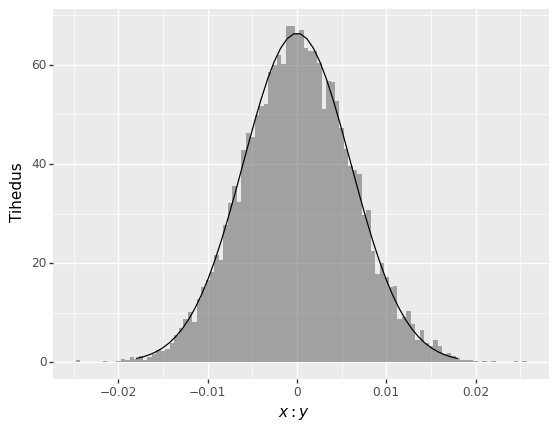
\includegraphics[width=0.8\textwidth]{jagatis_relatiivne_viga.png}
    \end{center}
    \caption{Jagatise $x:y$ relatiivse vea simuleeritud tihedus histogrammina ja teoreetiline lähendus normaaljaotsega juhul $x\sim\mathcal{N}(0{,}8; 0{,}004)$, $y\sim\mathcal{N}(0{,}9; 0{,}003)$.}
    \label{fig:jagatis relatiivne viga tihedus}
\end{figure}

Joonisel \ref{fig:jagatis relatiivne viga tihedus} on histogrammina esitatud simuleeritud jagatise $x:y$ relatiivne viga kümnetuhande juhuslikult genereeritud $x$ ja $y$ väärtuse puhul, kus $x\sim\mathcal{N}(0{,}8; 0{,}004)$, $y\sim\mathcal{N}(0{,}9; 0{,}003)$. Tumeda joonega on näidatud relatiivse vea lähendus normaaljaotusega tulemuse \eqref{eq:jagatis relatiivne viga dispersioon} põhjal.